\chapter{Computational details}
\label{sec:Computation}

This section is intended to provide the necessary details for reproduction of results to be presented later on. First we begin by describing the software used for the project. 

\section{Vienna Ab initio Simulation Package}
This software, often referred to as VASP is a package for ab initio quantum mechanics calculations using the projected augmented wave method and plane wave basis set. The intended methodology is DFT, but have been extended for methods post the original DFT-formulation. Calculations with VASP was carried out on the supercomputer fram, with allocated time and resources provided by Uninett Sigma2,\textbf{add reference!}.

The structure of VASP rely on a set of input files and output files from the calculation, the input files required to perform a DFT computation in VASP are the following:
\begin{itemize}
    \item INCAR - this file provide the tags responsible for different methods, algorithms, parameters etc.
    \item POSCAR - this file is related to the crystal structure of the system
    \item POTCAR - What psudopotential that is used
    \item KPOINTS - A file containing information on what KPOINTS will be used
    \item jobfile - This file contains information for the supercomputer regarding resources and such.
\end{itemize}
The capitalization displayed above is directly related to the requirements of the file system in the VASP/fram collaboration. Some important output files are:
\begin{itemize}
    \item CONTCAR - The relaxed crystal structure after finalized calculation
    \item CHGCAR - This file contains the electron density after calculation
    \item EIGENVAL - Contains the solutions to the Kohn-Sham eigenfunctions
    \item DOSCAR - Information on the Density of States
    \item OUTCAR - Contains a list of all other information.
\end{itemize}

\textbf{Some figure or tables to make this information more presentable}

In this project, we used the PAW psudopotential, and PBE GGA in favor of LDA for the reasons mentioned previously. Furthermore we readily employed meta-GGA functionals and hybrid-functionals, in particular SCAN and HSE06. We began the calculation of every individual structure by testing the convergence of total energy with respect to the number of k-points and cutoff energy. In VASP, the latter can be specified by setting the tag "ENCUT" in the INCAR file, we found 300 eV to yield productive results in terms of convergence and computation time for total energy calculations, and 400 for ionic+volume relaxations. Regarding the number of points in the reciprocal space, we carried out a great deal of simulations on numerous structures with distinct crystal structures and corresponding supercells, for this reason we employed a number of different sets of k-points depending on the structure. Typically the number of points ranged from a 2x2x2 mesh to 4x4x4 mesh. With the smaller being required for hybrid functionals to converge. 

Upon realizing the convergence parameters, the structures were allowed to relax both the ionic positions, and cell volume with the quasi-newton method and a convergence criterion of $1E-2$ for the forces and $1E-5$ for the total energy. However, the symmetry of the structure was forced constant by the use of vasp-std-noshear. This process was repeated two times before performing final total energy calculation with various functionals.

The specific tags, algorithms, parameters and options of VASP that was in use throughout this project can be found at our GitHub address, but in particular we would like to cover two specific parameters. The First is related to the magnetic configuration of our calculations, specified with the tag ISPIN in VASP. We used ISPIN=2 which allow for co-linear spin-polarized calculations due to the involvement of ferromagnetic elements such as iron and nickel in this study. However, there are many more magnetic orientations the system can adopt besides co-linear, therefore the final total energies we found may not be the true lowest energies. But given the allocated duration and resources of this project, this is a understood consequence. Secondly is the type of smearing that was used for the different calculations. The preferred method for accurate total energies and density of states in semiconductors is the tetrahedron method, and for accurate forces in metals the Methfessel-Paxton method is recommended. However, our system contains both metals and a large portion of Si. For this reason we used a combination of smearing methods. For the relaxation and minimization of forces, we used gaussian smearing with smearing width $\sigma = 0.05$, as this method provide accurate forces in both metallic and semiconducting materials. And to calculate the total energy and DOS, we used the tetrahedron method, as recommended. In order to obtain converged results of the HSE06 functional, we first calculated the charge density with gaussian smearing, then apply this density to perform a second hybrid calculation with the tetrahedron method. This was necessary becouse gaussion smearing yielded inaccurate and unreliable results in terms of the density of states when comparing to the band gap from the koh-Sham eigenvalues. However, this method, in addition to the narrow k-grid of just 2x2x2 k-points does include a factor of uncertainty regarding these results from the HSE06 functional. 


\textbf{This \cite{bandgap_vasp_forum} is a good reference for extracting the band gap of VASP jobs relating to smearing and DOSCAR vs EIGENVAL}

\textbf{Band structure/DOS and band-unfolding?}

\section{Generation of SQS}
\textbf{Needs work, add part on filling ratio of ideal cube}
The generation of special quasi-random structures as described in section .., was done by utilizing the Temperature Dependent Effective Potential (TDEP) method. This package, devolved by Olle Hellman, offers a wide range of tools primary intended for studies of finite temperature lattice dynamics. In this project we utilize the program generate-structure within the TDEP package to construct SQS's. The work of TDEP is the result of an unpublished PHD thesis by Nina Shulumba \textbf{(Insert citation)}, thus the documentation on the software and generate-structure script is limited, please refer to the original author for more information. 

In this project, we constructed SQS's by first transforming the cif-files of a given initial structure, for instance that of $FeSi_2$, to a primitive unit cell. The SQS's was generated by the same principles explained in section .., for each structure we created 5 distinct SQS's of an equal size under the constraint that the 3d atoms be distributed eqvimolar in the system. Precise file formats and such can be found at GitHub. Another approach could have been to construct SQS's of specific cell counts instead of total number of atoms, however this quickly lead to extremely large supercells, up to 256 atoms, that simply would not converge to our best efforts. 

We began by studying high-entropy silicides by alloying 3d-metal silicides such as $Fe_2Si$ by Cr, Fe, Co, and Ni to construct a $(CoCrFeNi)_2Si$ alloys. From this point we varied the distribution and type of elements in an attempt to locate high-entropy silicides with semiconducting properties, but remained within quaternary 3d silicides. Examples of SQSs generated by TDEP, from $FeSi_2$ structure with Cr, Fe, Mn and Ni can be seen in figure \ref{sqs_FeSi2}.

\begin{figure}
\begin{subfigure}{0.5\textwidth}
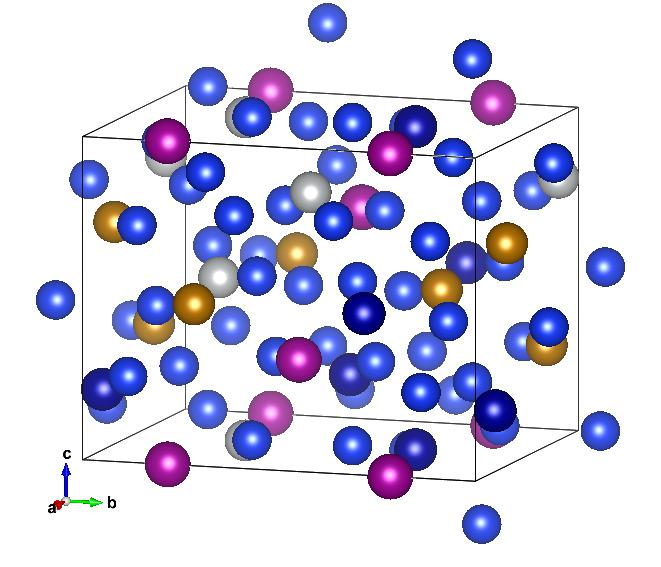
\includegraphics[width=\textwidth]{method/sqs/A.jpg}
\caption{Structure A}
\end{subfigure}
\hfill
\begin{subfigure}{0.5\textwidth}
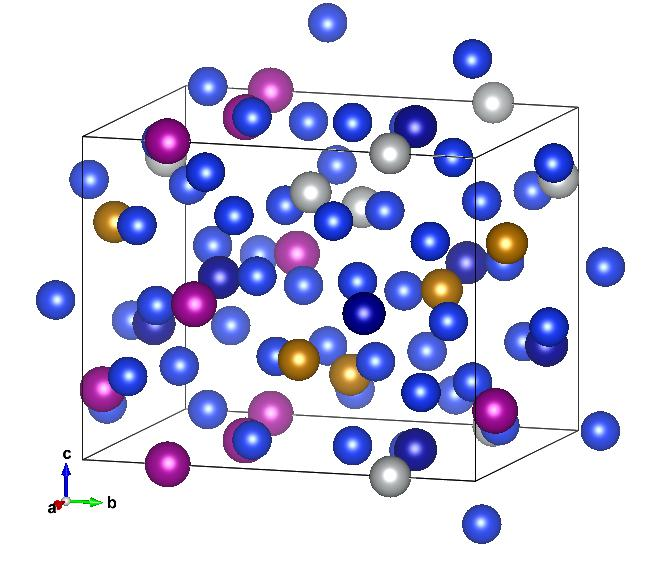
\includegraphics[width=\textwidth]{method/sqs/B.jpg}
\caption{Structure B}
\end{subfigure}
\begin{subfigure}{0.5\textwidth}
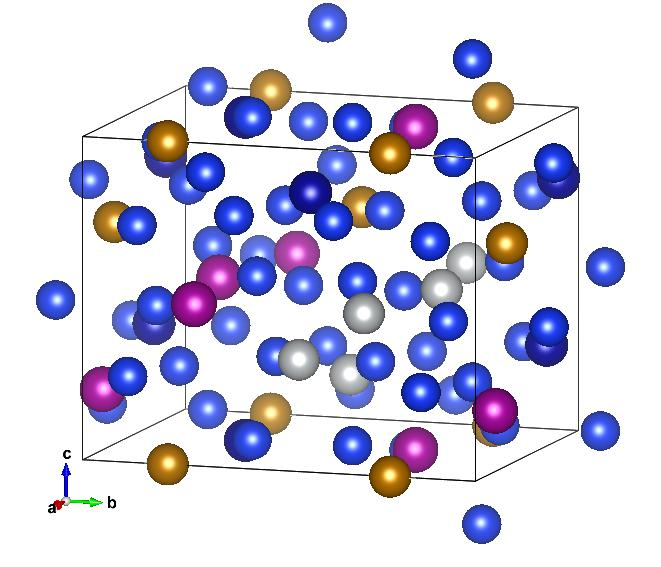
\includegraphics[width=\textwidth]{method/sqs/C.jpg}
\caption{Structure C}
\end{subfigure}
\hfill
\begin{subfigure}{0.5\textwidth}
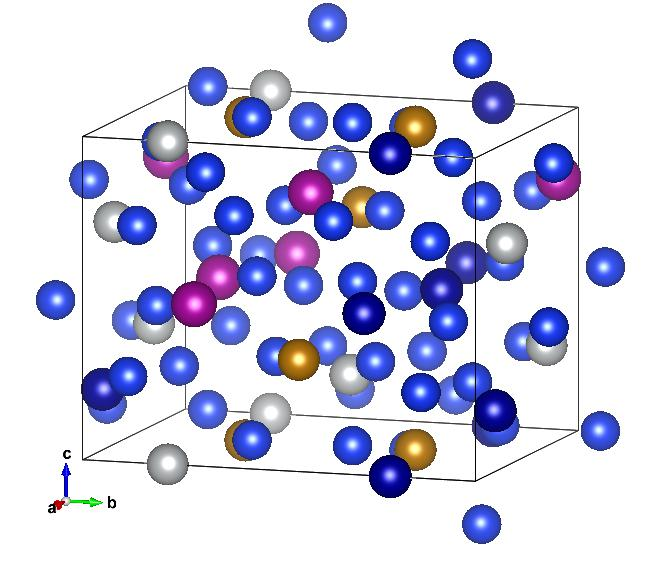
\includegraphics[width=\textwidth]{method/sqs/D.jpg}
\caption{Structure D}
\end{subfigure}
\begin{subfigure}{0.5\textwidth}
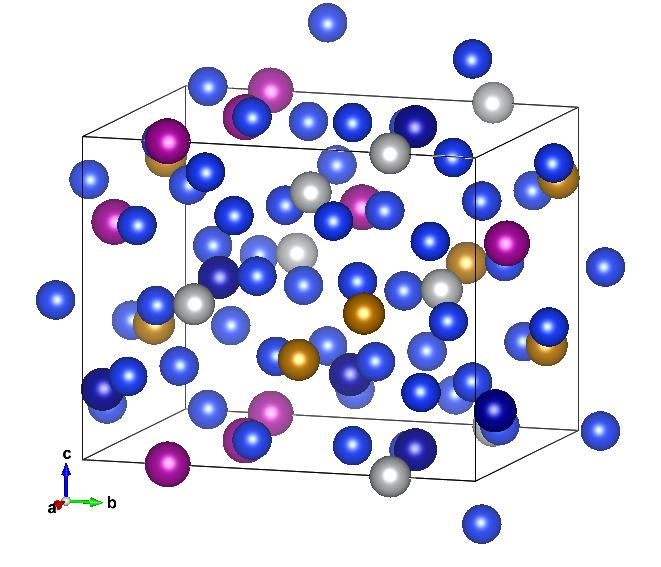
\includegraphics[width=\textwidth]{method/sqs/E.jpg}
\caption{Structure E}
\end{subfigure}
\caption{48 atom SQS based on eqvimolar distribution of Cr, Fe, Mn and Ni in and $FeSi_2$ cell.}
\label{sqs_FeSi2}
\end{figure}

\section{Band-structure?}

\section{Utility scripts}
During the course of the projects lifetime, several shell and python scripts was developed by myself and/or provided to me by my supervisor Ole Martin Løvvik and his team of researchers at Sintef. These can be located at the GitHub address :...